\documentclass[fleqn,12pt]{wlscirep}

%\newcommand{\charly}[1]{\textcolor{?}{#1}}
\definecolor{gainsboro}{rgb}{0.86, 0.86, 0.86}
\newcommand{\doing}[1]{\textcolor{gray}{#1}}
\newcommand{\todo}[1]{\textcolor{gainsboro}{#1}}
\newcommand{\red}[1]{\textcolor{red}{#1}}
\newcommand{\blue}[1]{\textcolor{black}{#1}}
\newcommand{\fig}[1]{\textcolor{black}{#1}}
\newcommand\note[1]{\mbox{}\marginpar{\footnotesize\raggedright\hspace{0pt}\color{orange}\emph{#1}}}

\usepackage{lineno}
\linenumbers
\usepackage{graphicx}

\let\oldthebibliography\thebibliography
\let\endoldthebibliography\endthebibliography
\renewenvironment{thebibliography}[1]{
  \begin{oldthebibliography}{#1}
    \setlength{\itemsep}{0em}
    \setlength{\parskip}{0em}
}
{
  \end{oldthebibliography}
}


\usepackage{hyperref}
\hypersetup{
     colorlinks   = true,
     citecolor    = black
}

\usepackage{parskip}
\setlength{\parskip}{6pt}
\setlength{\parindent}{0pt}
\renewcommand{\baselinestretch}{1.1} 

\usepackage{wrapfig}

\title{Quantifying plasmid dynamics using single-cell microfluidics and image bioinformatics}

\author[1]{JCR Hernandez-Beltran}
\author[2]{J Rodr\'iguez-Beltr\'an}
\author[2]{A San Mill\'an}
\author[1,*]{R Pe\~na-Miller}
\author[1,*]{A Fuentes-Hern\'andez}
\affil[1]{  \, Laboratorio de Biolog\'ia Sint\'etica y de Sistemas, Centro de Ciencias Gen\'omicas, Universidad Nacional Aut\'onoma de M\'exico, 62210, Cuernavaca, M\'exico}
\affil[2]{ \, Department of Microbiology, Hospital Universitario Ramon y Cajal (IRYCIS), Madrid, Spain}
\affil[*]{Corresponding authors: ayarifh@ccg.unam.mx, rpm@ccg.unam.mx}

\keywords{plasmid dynamics, fluorescence microscopy, image processing, microfluidics}

\begin{abstract}
\footnotesize{
Multicopy plasmids play an important role in bacterial ecology and evolution by accelerating the rate of adaptation and providing a platform for rapid gene amplification and evolutionary rescue. 
Despite the relevance of plasmids in bacterial evolutionary dynamics, evaluating the population-level consequences of randomly segregating and replicating plasmids in individual cells remains a challenging problem, both in theory and experimentally.
In recent years, technological advances in fluorescence microscopy and microfluidics have allowed studying temporal changes in gene expression by quantifying the fluorescent intensity of individual cells under controlled environmental conditions.
In this paper, we will describe the manufacture, experimental setup, and data analysis pipeline of different microfluidic systems that can be used to study plasmid dynamics, both in single-cells and in populations.
To illustrate the benefits and limitations of microfluidics to study multicopy plasmid dynamics, we will use an experimental model system consisting on {\em Escherichia coli} K12 carrying non-conjugative, multicopy plasmids ($19$ copies per cell, in average) encoding different fluorescent markers and $\beta$-lactam resistance genes. 
First, we will use an image-based flow cytometer to estimate changes in the allele distribution of a heterogeneous population under different selection regimes.  Then we will use a mother-machine microfluidic device to obtain time-series of fluorescent intensity of individual cells to argue that plasmid segregation and replication dynamics are inherently stochastic processes.  Finally, using a microchemostat, we track thousands of cells in time to reconstruct bacterial lineages and evaluate the \blue{allele} frequency distributions that emerge in response to a range of selective pressures.
}
\end{abstract}
\begin{document}

\flushbottom
\maketitle

%%%%%%%%%%%%%%%%%%%%%%%%%%%%%%%%%%%%%%%%%%%
\section*{Research highlights}

\begin{itemize}
    \item  Imaging can be used to study plasmid dynamics at multiple scales: from single-cells to bacterial populations 
    
    \item Intracellular plasmid dynamics is a noise-driven process resulting from randomly segregating and replicating plasmids.
    
    \item Selection modulates allele distributions by modifying the fraction of cells with different plasmid configurations.
    
    \item  Heteroplasmy is unstable in constant environments and stabilized in fluctuating environments.
    
\end{itemize}

\thispagestyle{empty}

\clearpage

%%%%%%%%%%%%%%%%%%%%%%%%%%%%%%%%%%%%%%%%%%%
\section{Introduction}
Plasmids are significant drivers of microbial ecology and evolution by horizontally transmitting beneficial genes and providing recipient cells with access to novel ecological niches\cite{wiedenbeck2011origins}. But the contribution of plasmids to bacterial evolutionary dynamics is not reduced to merely acting as vehicles for the horizontal dissemination of genetic information between strains and species.
Recent studies have enlisted a series of benefits associated with carrying genes in plasmids, as opposed to encoding them in the chromosome.

\blue{The fixation probability of beneficial mutations and the rate of segregational loss are determined by the number of plasmid copies carried by each cell\cite{stewart1977population} and, therefore, copy number control, as well as  and timing and mode of plasmid segregation, are important factors influencing the population genetics of plasmid-bearing populations \cite{paulsson2002multileveled,rodriguez2019genetic,Ilhan2019}.}
\blue{As a result, the stochastic nature of replication and segregation of multi-copy plasmids has been studied extensively, both in theory\cite{ishii1978random,nordstrom1984equipartition,keasling1989cole1,paulsson2001noise} and in laboratory conditions\cite{nordstrom1984control,novick1987plasmid,del2000plasmid}, showing that copy-number control is a noisy process with events randomly distributed in time \cite{seneta1983some} and, therefore, intracellular fluctuations in copy numbers can be seen as a stochastic dynamical system \cite{keasling1989cole1}. }

\blue{Similarly, plasmid partition is a random process such that, in the absence of plasmid addiction systems\cite{Mochizuki2006,baxter2015plasmid}, results in an equal chance for each plasmid to be inherited to each daughter cell and, therefore, in a binomial probability of producing a plasmid-free cell upon division. Of course, this is a simplification, as high-copy plasmids can produce dimers through homologous recombination\cite{summers1991kinetics} and intracellular spatial structure can result in the asymmetric segregation of plasmids upon division\cite{wang2016quantitative}. Also, low-copy plasmids tend to have active partitioning mechanisms that organize plasmids around a centromere-like site to segregate plasmids symmetrically between daughter cells at division.\cite{salje2010plasmid}. In contrast, plasmids that do not encode partition systems decrease the probability of segregational loss by being present in high-copy-numbers. }

\blue{But carrying multiple plasmid copies not only increases plasmid stability but can also have important consequences in the adaptive dynamics of plasmid-bearing populations, for instance increasing the rate of fixation of beneficial mutations \cite{galitski1995evidence} and accelerating the rate of adaptation to deteriorating environmental conditions\cite{san2016multicopy}. 
Furthermore,} once a beneficial mutation appears in a plasmid-borne gene, multicopy plasmids can provide a platform for rapid gene amplification \cite{nicoloff2019high}.  
By increasing gene dosage, bacterial cells have been reported to transiently enhancing the level of resistance to antibiotics\cite{santos2017naturally}, allowing the population to increase in size and, as a result, increasing the probability of appearance of secondary drug-resistant mutations\cite{Sun2018}. 

Moreover, multicopy plasmids produce genomic regions of local polyploidy that can generate heterozygous cells where different alleles coexist at a cellular level, a phenomenon also referred to as heteroplasmy\cite{novick1987plasmid}. As a result, individual cells can increase their genetic diversity and enable populations to circumvent evolutionary trade-offs\cite{Rodriguez2018}.
It has also been reported that the multicopy plasmids can increase standing genetic variation in the population, thus enabling bacterial populations to escape extinction following a sudden environmental change\cite{santer2019evolutionary}. 
In the absence of selection, however, random genetic drift of multicopy plasmids during cell division (also known as segregational drift\cite{Ilhan2019}) can reduce the rate of adaptation, despite high-copy plasmids having increased mutational supply.

By focusing on large population sizes, laboratory studies have been able to characterize the interaction between genetic dominance and strength of selection, and correlate these traits with the probability of fixation of mutant alleles and the horizontal transmission of plasmid-borne genes\cite{rodriguez2019genetic}.
Other plasmid evolution studies have focused on compensatory adaptation\cite{SanMillan2014,Wein2019,hall2020extremely}, horizontal transmission\cite{Lopatkin2017} and co-evolution between hosts and plasmids\cite{Harrison2015}.
Altogether, these results highlight the complex interaction between the intracellular plasmid dynamics and the evolutionary dynamics of bacterial populations. 

\subsection{\blue{Single-cell microfluidics}}

In the past decades, biology and medicine have been rapidly evolving towards using quantitative tools to study complex biological systems. Interdisciplinary studies use statistical, mathematical, and computational tools, combined with experimental and molecular biology, to understand the behavior of individual cells within a population \cite{artemova2015isolated} and to predict their response to environmental change\cite{el2018heterogeneity}. The benefit of implementing a {\em bottom-up} approach is that we can follow the life history of individual cells, instead of averaging large populations and making inferences about cellular processes from population-level observations.

\blue{Fluorescence microscopy has been previously used to estimate plasmid copy-numbers\cite{ng2010plasmid,lobner1999distribution}, as well as to visualize conjugation\cite{babic2008direct}, to study horizontal transmission of plasmids\cite{del2012determination} and to explore the range of different plasmid-host associations\cite{shintani2014single}. It has also been used to evaluate {\em in situ} conjugation in bacterial plant endosymbionts\cite{banuelos2019conjugative} and horizontal gene transfer in microbiomes\cite{pinilla2018monitoring}.
Moreover, with the use of fluorescent probes, microscopy studies have been able to study with great detail the spatio-temporal distribution of plasmids inside a cell, as well as the segregation dynamics occurring upon division\cite{Reyes2013,Hsu2019,wang2016quantitative}.  These single-molecule studies, however, only consider a small set of cells and are constrained to short-term experiments in constant environments.}

\blue{On the other hand, microfluidic devices have been used in combination with fluorescence to obtain time-series of gene expression of individual cells \cite{Young2012,tomanek2020gene}.  Microfluidic devices can be fabricated using soft lithography \cite{zhang2012inkjet,pan2011maskless}, micro-droplets \cite{boedicker2009microfluidic} and protein-based micro-3D printing \cite{connell2014real}. In general, the goal of these devices is to restrict the movement of bacterial cells to observe them for long time intervals with the aim of studying, for instance, gene expression dynamics\cite{Young2012,baumgart2017synchronized,bennett2009microfluidic,locke2009using}, as well as to evaluate the consequences of asymmetric division and cell-to-cell variability of key cellular processes \cite{mosheiff2017correlations,bergmiller2017biased,el2018heterogeneity}.
A brief overview of different microfluidic devices and their uses can be found in \cite{bennett2009microfluidic,potvin2018microfluidics}. }

\blue{A myriad of computer vision algorithms have been developed to analyze time-lapse movies acquired using a fluorescent microscope\cite{Young2012,vanValen2016,Berg2019,balomenos2017image,arnoldini2014bistable,sachs2016image,lugagne2019delta,kamentsky2011improved}.  Of note, {\em Schnitzcell}\cite{Young2012} was designed to study colonies of rod-shaped bacteria (e.g. {\em Escherichia coli} and {\em Bacillus subtilis}) growing in agar pads, although it is not longer maintained.  Recently, novel computational techniques based on machine learning have been successfully incorporated into bio-image analysis pipelines. For example, {\em DeLTA}\cite{lugagne2019delta} and {\em DeepCell}\cite{vanValen2016} implement deep convolutional neural networks to perform accurate segmentation and lineage reconstruction, while {\em Ilastik}\cite{berg2019ilastik} provides a user-friendly suite for image segmentation and cell tracking. }

\blue{Besides quantifying single-cell fluorescent intensity, imaging algorithms can also be used to record division events and to estimate duplication and elongation rates of individual bacterial cells.  In consequence, microfluidics have been used to study cell growth and homeostasis\cite{wallden2016synchronization}, senescence\cite{ackermann2003senescence,lindner2008asymmetric} and bacterial adaptation to stress\cite{lapinska2019bacterial,mathis2016response,patange2018escherichia}. By correlating physiological and morphological properties of individual cells with the level of expression of a gene of interest, previous studies have shown that phenotypic heterogeneity can provide functional benefits for bacterial populations, for instance allowing the implementation of division of labor strategies or increasing survival of the population to fluctuating environmental conditions\cite{Ackermann2015}.
Another benefit of single-cell microfluidics is that it allows us to estimate growth rate differences and survival rates in response to environmental change.  Therefore microfluidics has been proposed as a strategy for rapid antimicrobial susceptibility determination \cite{Baltekin2017,Aroonnual2017} and to study gene regulatory changes that emerge in response to genetic and environmental perturbations\cite{rochman2016grow,chait2017shaping}.   }

In this paper, we combine microfluidics, fluorescent microscopy, and computer vision algorithms to study the interaction between multicopy plasmids and bacterial fitness in dynamic environments. To achieve this goal, we use a previously characterized experimental system consisting of plasmid-mediated $\beta$-lactam resistance evolution in {\em Escherichia coli}\cite{Rodriguez2018}. The objective of this manuscript is to describe the use fluorescence and multiple image-based technologies to identify the source of noise in the replication and segregation dynamics of multicopy plasmids, as well as to evaluate the effect of selection imposed by antimicrobial substances on the distribution of plasmids exhibited by single-cells and bacterial populations.
 
%%%%%%%%%%%%%%%%%%%%%%%%%%%%%%%%%%%%%%%%%%%
\section{Material and methods}

%%%%%%%%%%%%%%%%%%%%%%%%%%%
\subsection{Bacterial strains and plasmids}

In this study, we use derivatives of \textit{Escherichia coli} MG1655 strains previously published \cite{san2016multicopy,Rodriguez2018}. In short, a $\beta$-lactamase gene $bla_{\text{TEM-1}}$ that confers resistance to ampicillin (AMP) was inserted into a small non-transmissible multi-copy plasmid p3655 derived from pSU18T and pBADgfp2, with a ColE1-like (p15a) origin of replication\cite{le2007construction}, a plasmid referred to in this study as pBGT-1.  This plasmid also contains an eGFP gene under an arabinose promoter with an {\em araC} repressor. Another plasmid, pBRT,  was derived from pBGT by replacing the $bla_{\text{TEM-1}}$ gene with $bla_{\text{TEM-12}}$, a TEM variant that confers resistance to ceftazidime (CAZ) and mild resistance to ampicillin (AMP). Also, eGFP was replaced by a DsRed gene, and the native {\em cat} resistance gene was knocked-out. In this study, we refer to heterozygous cells simultaneously carrying both plasmids as HT, while G1 and R12 denote homozygous cells bearing pBGT-1 and pBRT-12, respectively (see \fig{Fig \ref{fig:experimental_system}A} for maps of these plasmids). It is important to emphasize that pBGT-1 and pBRT-12 share an origin of replication and only differ in the fluorescent marker and the TEM variant carried. Therefore the plasmid copy-number control mechanism regulates the maximum number of plasmids carried in each cell, independently of the plasmid type.

%%%%%%%%%%%%%%%%%%%%%%%%%%%
\subsection{Media and growth conditions}

Experiments were performed using Lysogeny Broth- Lenox (LB) (Sigma-L3022) supplemented with arabinose (0.5\% w/v). 
Antibiotic minimum inhibitory concentrations (MIC) were calculated using standard dose-response curves. 
To balance HT cells, we prepared the overnight culture using LB media supplemented with 15 mg/l of chloramphenicol and 0.5 mg/l ceftazidime. 
Stocks solutions at 20\% of Arabinose (Sigma-A91906) were prepared by diluting 2g of arabinose in 10ml DD water sterilized by filtration. 
AMP stock solutions (100mg/ml) were prepared by diluting ampicillin (Sigma-A0166) directly in LB and adding arabinose (0.5\%). Stock solutions of ceftazidime (Sigma-A6987) were diluted in water at 10 mg/ml and sterilized by filtering. Chloramphenicol (Sigma-C0378) stock solutions were prepared at 50 mg/ml in ethanol (97\%).   
Population-level experiments were performed using 20 ml of LB media in 125 ml titration flasks. Three replicates of HT cells cultures were grown in balancing media for 24 hours in a shaker incubator at 37$^{\circ}$ C and 200 rpm. 

%%%%%%%%%%%%%%%%%%%%%%%%%%%
\subsection{Imaging flow cytometry}

Population-level experiment measurements were performed by sampling 1ml of overnight culture and measured their fluorescence using an imaging flow cytometer (Amnis ImageStream Mark II by Luminex). INSPIRE software was used to acquire data discriminating by area, aspect ratio, focus, and side scatter features. GFP fluorescence was excited at 488 nm with 25 mv intensity, and DsRed fluorescence was excited at 561 nm with 200 mv intensity. Populations data files were processed using IDEAS 6.2 software and feature values were exported and analyzed using bespoke scripts implemented in Python programming language. 
%%%%%%%%%%%%%%%%%%%%%%%%%%%
\subsection{Microfluidic devices}

We used PDMS (polydimethylsiloxane) microfluidic chips obtained from wafers manufactured using soft photolithography (SU-8 2000.5, micro resist technology GmbH).
In particular, we used a micro-chemostat \cite{mondragon2011entrainment} that contains multiple inputs (a cell-loading input, a shunt, and two for different growth media), as well as two waste outputs. Media inputs are mixed at different proportions using a red fluorescent dye (rhodamine) diluted in one of the media inputs. This device contains 48 chambers of $40x50x.95$ $\mu$m, capable of trapping approximately $500$ bacterial cells in the same focal plane.  
Each chamber is open to a big channel on two sides and, when chambers are filled, bacteria in the edges are pushed out of the chamber and washed away. We use this device to obtain high-throughput population-level data derived from single-cell measurements at different time-points.
We also used a dual-input mother-machine \cite{Kaiser2018} device in which bacteria are trapped in a comb-like channels architecture. Mother cells restrained at the bottom of each channel and, as they grow and divide, daughter cells are pushed downwards to a larger channel and washed away. We use this microfluidic chip to keep track of mother cells for very long periods of time, while quantifying fluorescence and other morphological attributes.

%%%%%%%%%%%%%%%%%%%%%%%%%%%
\subsection{Cell loading and environmental control}

Growth media was loaded into $60$ml-syringes connected to the PDMS chip through Tygon tubes and assorted Luer connectors. The pressure inside the chip is controlled with vertical linear actuators and a digital signal generator that controls the height of each syringe. 
This Dial-A-Wave (DAW) system\cite{Ferry2011} enables precise control over the extracellular environmental conditions. For the purpose of this paper, we use this DAW to introduce antibiotics into the chip gradually, until reaching a maximum dose that is then maintained until all cells are killed, a protocol we refer to as a ramp experiment.  Later we will introduce antibiotics following a sinusoidal signal to alternate selective pressures periodically.

Initial inoculates of HT cells were grown overnight in the presence of sub-lethal doses of chloramphenicol and ceftazidime, in order to clear homozygous cells from the culture and obtain a well-balanced HT culture.
A sample was then transferred to $200$ml of fresh LB and grown at 30$^{\circ}$C until reaching an OD$_{600}=0.3$.  After centrifuging, cells were re-suspended in $5$ml of LB, and this dense culture was used to inoculate the microfluidic chip. For all microfluidics experiments, we used LB media supplemented with arabinose at $0.5$\% and Tween20 ({Sigma-P2287}) at $0.075$\%. In all cases, cells were allowed to grow and divide multiple cell cycles in a drug-free environment, allowing us to determine the baseline fluorescent intensity of the population. We later use this value to normalize our data and compare fluorescent intensities obtained for different channels.

%%%%%%%%%%%%%%%%%%%%%%%%%%%
\subsection{Microscopy and image acquisition}

Time-lapse images of microfluidic experiments were acquired using a Nikon Eclipse Ti-E epifluorescence microscope equipped with differential interface contrast (DIC), a motorized stage and a perfect focus system that allows us to obtain long-time time-lapses. The microscope was controlled by the Nikon NIS-Elements AR 4.20 program and is equiped with a Lexan Enclosure Unit with Oko-touch temperature control that allows us to incubate the microfluidic chips. The experiments are conducted at 30$^{\circ}$C.
For all experiments, time-lapse movies were acquired with a 100X Plan APO objective without analog gain and with field and aperture diaphragms as closed as possible to avoid photobleaching. DIC images were taken at 9v DIA-lamp intensity with exposure of 200 ms, DsRed channel (excitation from 540 to 580 nm, emission from $600$ to $660$ nm filter) with exposure of 600 ms, GFP channel (excitation from $455$ to $485$ nm, emission from $500$ to $545$) with $300$ ms exposure. Images were taken every 5 or 10 minutes, depending on the experiment. 


%%%%%%%%%%%%%%%%%%%%%%%%%%%%%%%%%%%%%%%%%%%
\subsection{Image processing and analysis}

Microscopy time-lapse movies were analyzed using a semi-automated ImageJ \cite{schneider2012nih} analysis pipeline that implements a deep-learning algorithm for image segmentation \cite{vanValen2016}.  Cell tracking and lineage reconstruction were performed in Python using standard numerical and geometric libraries (NumPy, Shapely, Pandas, Scipy, Matplotlib).  Data and code are openly distributed and available for download at \href{https://github.com/ccg-esb-lab/uJ}{https://github.com/ccg-esb-lab/uJ}.

 In short, the image processing pipeline consists on 1) organizing TIF files generated by NIS Elements, 2) aligning traps and using rigid motion transformation to correct for x-y drift in time-lapse images, 3) using {\em Parallel Interactive Deconvolution} with a theoretical point spread function generated with PSF Generator to produce a segmentable image, 4) using {\em DeepCell}\cite{vanValen2016} to segment images and obtain binary masks, 5) cell detection and automatic correction of ROIs, 6) manual correction of a binary mask, 7) data acquisition by overlapping masks in different fluorescent and bright field channels, 9) cell tracking using a feature-aided nearest-neighbor algorithm and lineage reconstruction and, finally, 10) data analysis and visualization.
The goal of this image bioinformatics pipeline is to acquire time-series of fluorescent intensity and other morphological properties of individual cells, as well as to obtain population-level statistics to estimate, for instance, the mean cell duplication rate of the population or changes in the shape of the fluorescence distribution.

%%%%%%%%%%%%%%%%%%%%%%%%%%%%%%%%%%%%%%%%%%%
\subsection{Estimation of plasmid copy-number and plasmid frequency}

There are two quantities we estimate from fluorescent data: plasmid copy-number (PCN) and plasmid frequency (PF). 
Previous studies have established that gene copy-number and fluorescent intensity are positively correlated, both when carried in chromosomes\cite{bergmiller2017biased} or in plasmids \cite{ghozzi2010inference,Rodriguez2018}.  Therefore we will use flow cytometry and fluorescent microscopy to determine the relative intensity of individual cells with respect to the population-level mean (it was previously determined that the plasmids used in this study are carried, on average, $\sim 19$ copies of the plasmid per cell)\cite{san2016multicopy}. 

Also, we estimate the proportion of each plasmid type carried in each cell from the relative fluorescent intensity measured on different channels.  
Let us define $\Phi_g$ and $\Phi_r$ the fluorescent intensity of cell $i$ measured in the green and red channels, respectively.  As fluorescent proteins have different maturation times and intrinsic brightness\cite{Balleza2018}, we normalized the data by dividing every channel measurements by the maximum intensity and obtained relative intensity values for each channel, quantities that we will denote as $\hat{\Phi}_g$ and $\hat{\Phi}_r$.  

We argue that, in this case, a polar representation of fluorescent data is more appropriate, as illustrated in the diagram shown in \fig{Figure 1B}.
That is, to estimate plasmid fraction from flow cytometry or microfluidic data we will transform the $\hat{\Phi}_g/\hat{\Phi}_r$ ratio into polar coordinates:
\begin{align*}
    PF \sim \theta &:=\arctan(\hat{\Phi}_r/\hat{\Phi}_g).
\end{align*}
\blue{This expression allows us to estimate the fraction of plasmids (PF), pBGT-1 plasmid  with respect to the pBRT-12 plasmid, a quantity we refer to as {\em relative fluorescent intensity} and denote as $\theta$. Similarly, we can use $r$ to approximate the absolute plasmid copy number (PCN) by assuming that fluorescent intensity is proportional to the number of copies of the gene carried by each cell,  
\begin{align*}
    PCN \sim r&:=\sqrt{\hat{\Phi}_g^2+\hat{\Phi}_r^2}.
\end{align*}
However, the assumption of a linear relationship between PCN and absolute fluorescent intensity does not always hold and, as discussed extensively in \cite{tal2012evaluating}, prevents from using absolute fluorescent intensities as a proxy for plasmid copy number.  For this reason, in this paper we will restrict our analysis to using $\theta$ to evaluate changes in the relative abundances of each allele (i.e. the plasmid fraction) in response to different environmental conditions.} 

%%%%%%%%%%%%%%%%%%%%%%%%%%%%%%%%%%%%%%%%%%%
%%%%%%%%%%%%%%%%%%%%%%%%%%%%%%%%%%%%%%%%%%%

%%%%%%%%
%%Figure 1 - Experimental system
\begin{figure}[ht!]
\centering
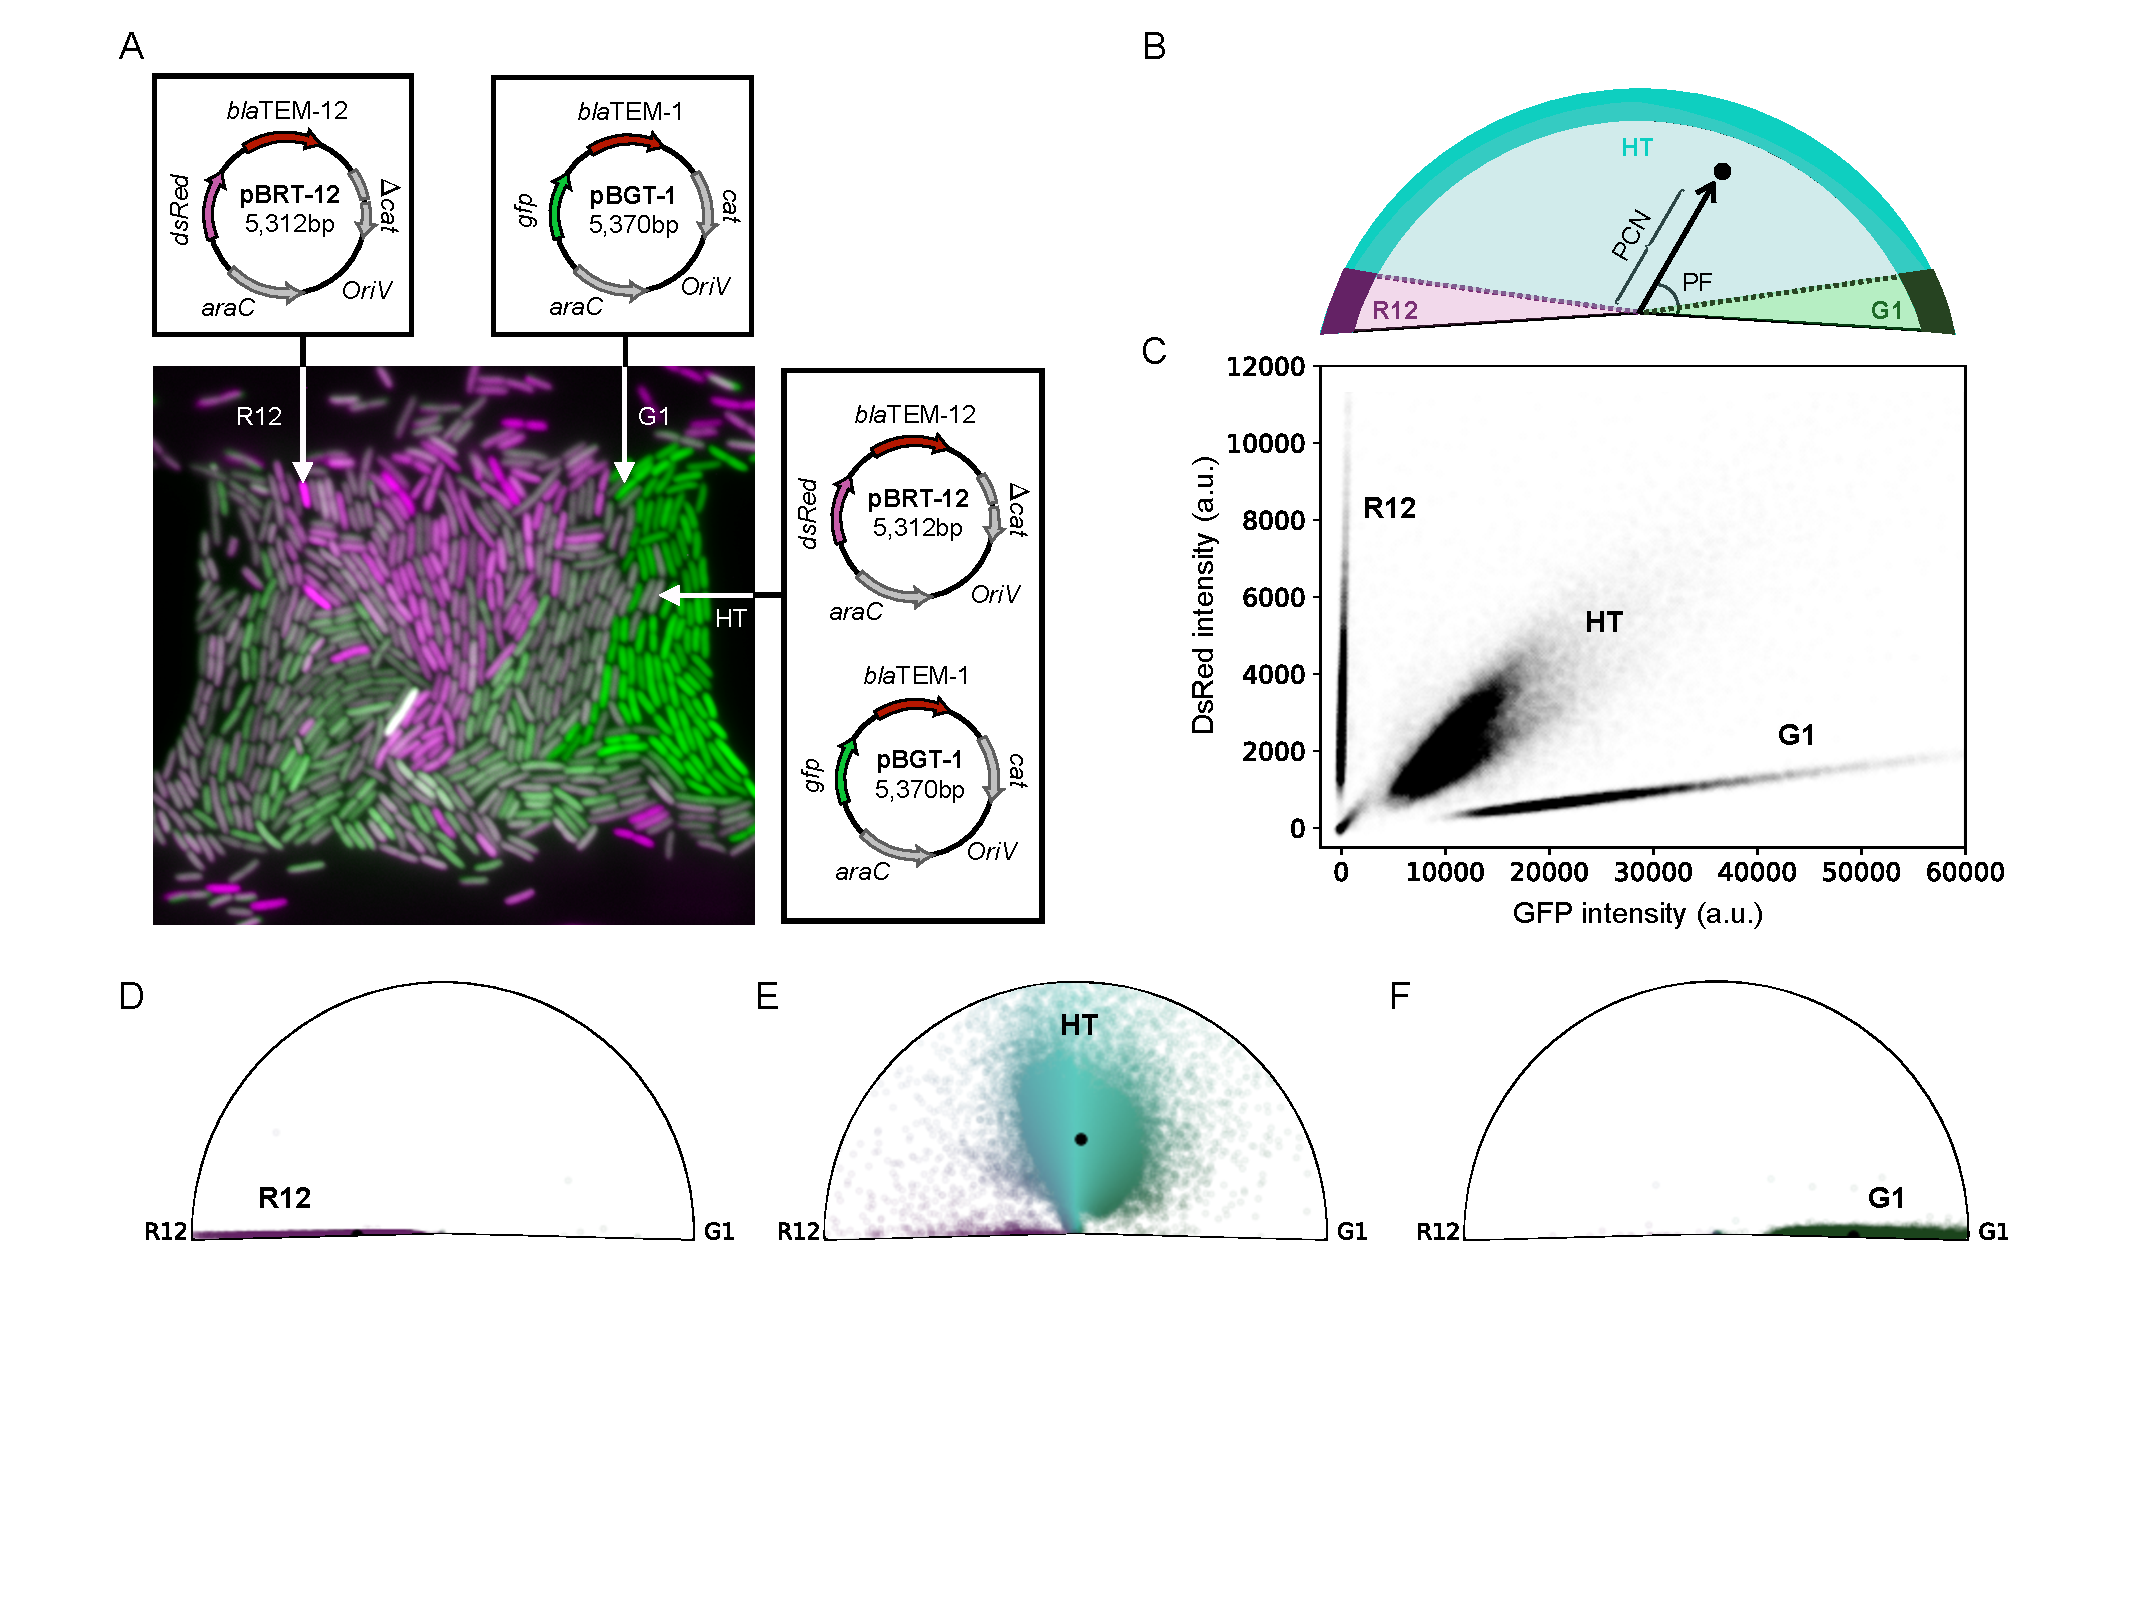
\includegraphics[width=\linewidth]{figures/Figure1.pdf}
\caption{ \small{A) Maps of plasmids used in this study. Composite microscopy image shows a heterogeneous {\em E. coli} population composed of cells carrying only pBRT-12 (denoted as R12, in magenta), pBGT (G1, in green) and a combination of both plasmids (HT).  B) Diagram illustrating a polar representation of multi-channel fluorescent data.  After normalizing fluorescence intensities obtained in GFP and DsRed channels, each cell can be represented as a point in a  two-dimensional polar coordinate system, where the relative fluorescence between DsRed and GFP channels can be approximated by an angle and the absolute fluorescence intensity from its distance to the origin.  We argue that absolute fluorescence is correlated with plasmid copy-number (PCN) and relative fluorescence to the plasmid fraction (PF). C) Raw cytometry data of a heterogeneous population illustrates that a flow cytometer can be used to identify different subpopulations, namely R12, G1 and HT. D-F) Polar representations of different plasmid-bearing populations n drug-free media: D) cells carrying only pBRT-12, E) a heterozygous population where both plasmids co-exist at a cellular level, and F) homozygous cells with only pBGT-1. Black dotes denote the expected value of the corresponding plasmid copy-number distribution}} 
\label{fig:experimental_system}
\end{figure}
%%%%%%%%


\section{Results}

%%%%%%%%


%%%%%%%%%%%%%%%%%%%%%%%%%%%%%%%%%%%
%%%%%%%%%%%%%%%%%%%%%%%%%%%%%%%%%%%
\subsection{Using flow cytometry to study population dynamics of heterogeneous populations}
A fundamental problem in plasmid biology is to determine environmental conditions that enable costly plasmids to be stably maintained in bacterial populations\cite{Harrison2015,loftie2016evolutionary,porse2016survival}. This problem is of particular interest for bioengineers and synthetic biologists, as genetic manipulations of microorganisms generally use plasmids as cloning vectors, despite being metabolically costly and, therefore, susceptible to be lost through purifying selection.  In contrast, as drug-resistant genes tend to be carried in plasmids \cite{alekshun2007molecular,san2018evolution}, it is also a problem of interest for biomedical scientists to determine conditions that cure drug-resistant plasmids of pathogenic populations\cite{boucher2009bad} and to evaluate the probability of fixation of drug-resistance mutations\cite{Ilhan2019,Rodriguez2018}.  

Independently of the motivation, experimental studies routinely estimate the fraction of plasmid-bearing cells within a bacterial population by replicating bacterial colonies from non-selective agar plates onto plasmid-selective and non-selective media. 
In recent years, other studies have used a combination of flow cytometry (FCM) and real-time quantitative PCR (qPCR) to estimate the mean plasmid copy number of the population\cite{ng2010plasmid} and to determine the relative abundance of plasmid-bearing cells\cite{bahl2004quantification}.  The benefit of the FCM and qPCR is that both are cultivation-independent and provide precise estimations about the mean plasmid copy number of the population. 

Here we use an image-based FCM (see Methods) to study the resulting PCN distribution that emerges from exposing genetically-diverse populations to different selection regimes. We focus on a well-characterized experimental system of drug resistance evolution: plasmid-mediated TEM-1 evolution towards ceftazidime resistance in {\em Escherichia coli}. The numerous ways in which TEM has evolved suggests that it can respond very specifically to each $\beta$-lactam, and therefore has been used extensively to study the molecular evolution in response to different selection regimes, both when TEM is encoded in the chromosome \cite{Barlow2002, Barlow2003} or in plasmids \cite{Rodriguez2018,santos2017naturally}.  
Indeed, nearly every $\beta$-lactamase that has been identified as a resistance determinant among clinical bacteria has experienced molecular evolution in response to the use of different $\beta$-lactam antibiotics, with over 215 variant TEM $\beta$-lactamases identified with differences in amino acid sequence and susceptibility to $\beta$-lactam antibiotics\cite{Barlow2002}.


%%%%%%%%%%%%%%%%%%%%%%%%%%%%%%%%%%%
\subsubsection{\blue{Relative allele frequencies} are modulated by selection and segregational drift}
Our experimental systems consists \blue{of} a bacterial population containing small ($5.3$Kb), non-conjugative, multicopy plasmids (pBGT with mean PCN=$19.12\pm1.56$, and pBRT with $21.1\pm0.85$ plasmids \blue{in} average\cite{san2016multicopy}), different fluorescent markers (GFP and DsRed respectively, both under the {\em araC} promoter) and TEM genes that produce different variants of $\beta$-lactamase, an enzyme that hydrolyzes the active portion of $\beta$-lactam antibiotics \cite{Knox1995}. 

\blue{It has been established there is a fitness cost associated with synthesizing fluorophores, in this case, expressed in terms of a reduced growth rate in the presence of arabinose with respect to the same strain growing in arabinose-free environments (two-tailed t-test, p-value$<0.05$, $N=4$). For this reason, all experiments described in this study were performed in the presence of arabinose. Crucially, both fluorescent proteins impose a similar fitness burden and therefore no significant differences in growth rate were observed in populations producing either GFP or DsRed proteins (two-tailed t-test, p-value$=0.512$, $N=6$)\cite{SanMillan2014}, therefore allowing us to associate changes in fluorescent intensity to differences in fitness of the corresponding TEM alleles, and not due to differential cost of producing fluorescent proteins.}

\fig{Figure 1A} displays a composite microscopy image showing that a population of HT cells presents high levels of heterogeneity; while some cells are only detected in DsRed or GFP channels (corresponding to cells with high proportions of either plasmid), other cells exhibit analogous levels of fluorescence in both channels (corresponding to heterozygous cells bearing both pBGT-1 and pBRT-12, mean(PCN)=$22.3 \pm 4.7$).  \fig{Figure 1C} shows raw fluorescent intensity determined with flow cytometry of cells in a heterozygous population, revealing the existence of three main clusters, corresponding to homozygous cells (R12 and G1) and the heterozygous population (HT).  \blue{All flow cytometry experiments were performed in triplicate, with fluorescence distributions obtained by sampling 20,000 cells from the corresponding population.}

 \fig{Figures 1D} and \fig{1F} show that clonal populations of G1 and R12 are only present in the corresponding region of the polar coordinate system when measured after 24 hours of growth.  
In contrast, HT cells carry both plasmids and are therefore scattered throughout the polar plane. This large dispersion in PCN and PF has been predicted by theoretical models of multicopy plasmid dynamics \cite{pena2015evaluating, Munch2019}, suggesting that populations bearing multicopy plasmids can present cell-to-cell differences in total plasmid copy-number and in plasmid frequency. 
Indeed, recent clinical studies have suggested that gene amplification and copy-number variability in drug-resistance genes yield heteroresistant populations\cite{andersson2019mechanisms}, potentially leading to treatment failure in clinical settings \cite{nicoloff2019high,wang2014heteroresistance, band2019heteroresistance}.

%%Figure 2- AMNIS
\begin{figure}[ht!]
\centering
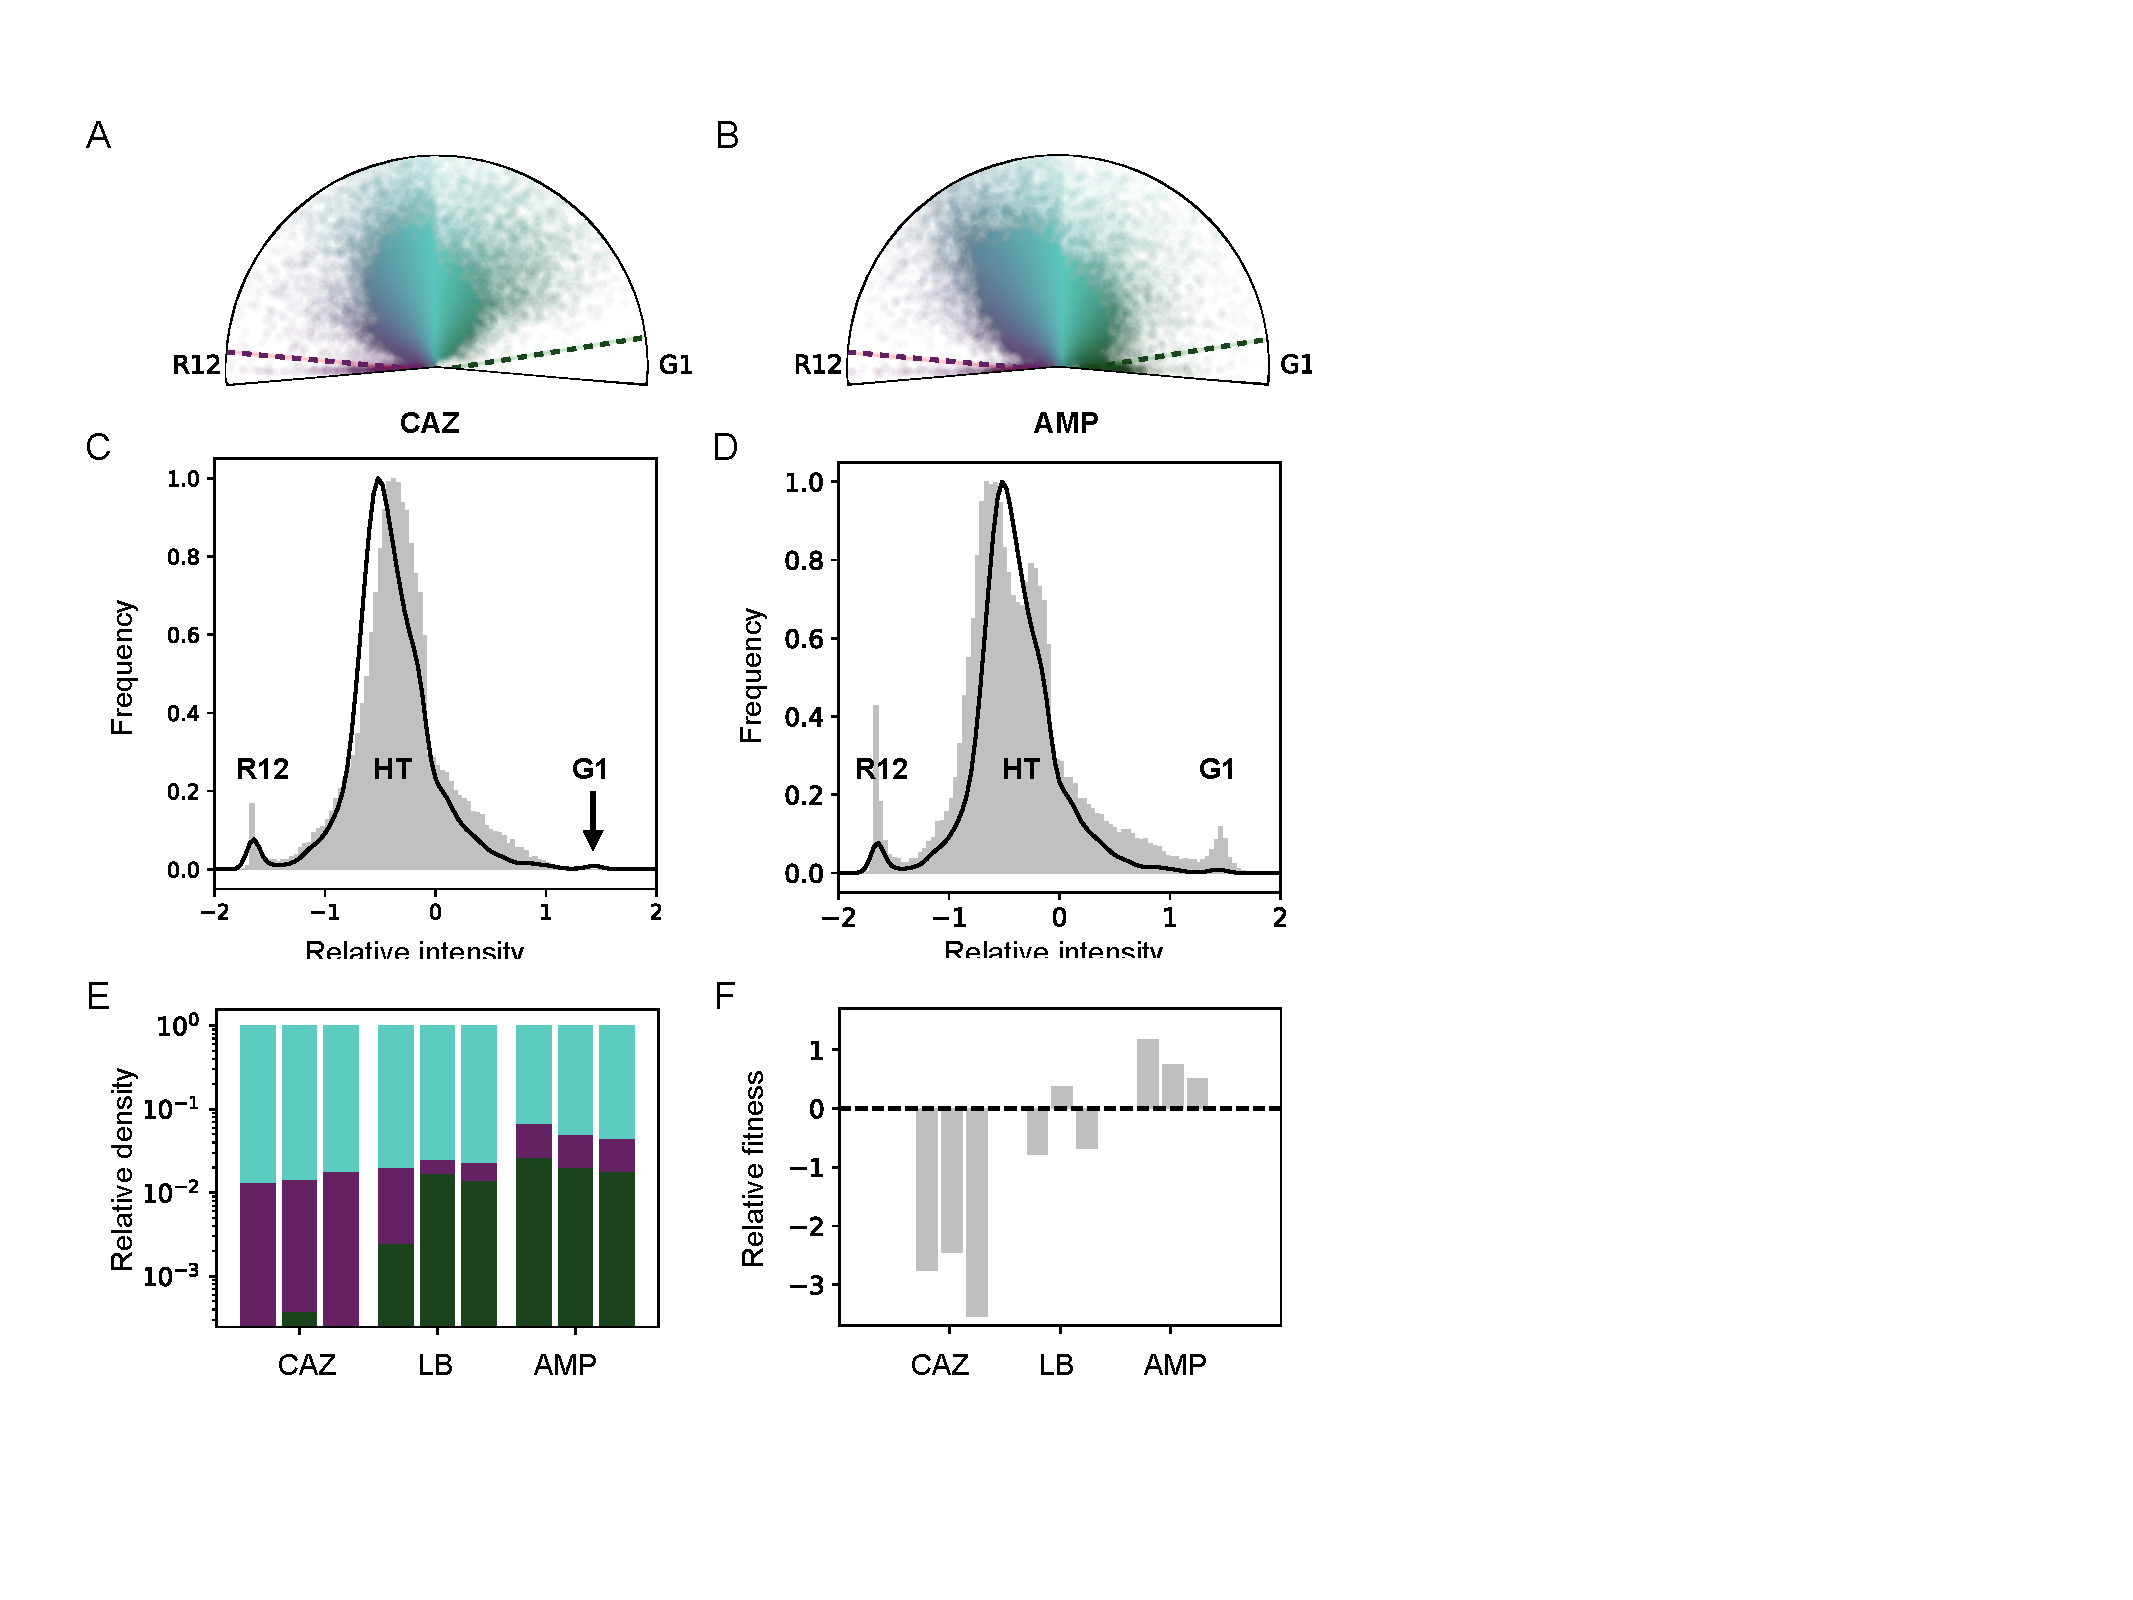
\includegraphics[width=.66\linewidth]{figures/Figure2.pdf}
\caption{ \small{ Polar representation of fluorescent intensities obtained using flow cytometry of HT populations exposed to A) ceftazidime, and B) ampicillin. \blue{Distributions were obtained by sampling 60,000 cells from three independent biological replicates.}  C-D) Histograms of relative intensity for both selection regimes, CAZ and AMP, respectively.  Note how AMP maintains a subpopulation of G1 cells, while in CAZ, only HT and R12 cells are present at the end of the experiment \blue{(the arrow in C points towards relative intensity values that correspond to G1)} . This is a consequence of R12 cells being resistant to both antibiotics and G1 only resistant to AMP. In drug-free media, both homozygous populations are present, resulting from the segregation of HT cells into G1 or R12. E) The relative density of each subpopulation under different environmental conditions, determined by clustering cells according to their relative fluorescent intensity. \blue{Each bar corresponds to a replicate experiment in each environment (N=3).} F) Relative fitness of G1 with respect to R12, after 24 hours of growing under different environmental conditions \blue{(N=3)}. As expected, AMP provides a fitness benefit for G1, while CAZ positively selects for R12. }}
\label{fig:AMNIS}
\end{figure}
%%%%%%%%

A consequence of bearing plasmids with different variants of TEM is that heterozygous populations exhibit heterogeneous profiles of resistance.  In this case, $bla_{\text{TEM-1}}$ provides resistance to ampicillin (AMP), while $bla_{\text{TEM-12}}$ to ceftazidime (CAZ) and partially to AMP\cite{Rodriguez2018, mroczkowska2008fitness}. 
So, to determine how different environments modulate the distribution of plasmids, we inoculated a population of HT cells in drug-free media and, after 24 hours, used a flow cytometer to obtain the distribution illustrated in Figure \ref{fig:experimental_system}E.
Similarly, we exposed a heterozygous population to a sub-lethal concentration of ampicillin ($8 mg/ml$) and estimated the resulting plasmid distribution after 24 hours (see \fig{Figure \ref{fig:AMNIS}A}). We then repeated this assay with ceftazidime ($8 \mu g/ml$) and, analogous to AMP,  HT cells exhibited large dispersion, while R12 and G1 showed variability in PCN, but not in PF. 

We then clustered the population based on their relative fluorescent intensities and counted the number of cells in each group. The relative abundances of each subpopulation are illustrated in \fig{Figure \ref{fig:AMNIS}E}. Note how, in drug-free media, segregational instability produces homozygous subpopulations, either carrying $bla_{\text{TEM-1}}$ or $bla_{\text{TEM-12}}$.
As $bla_{\text{TEM-1}}$ is susceptible to ceftazidime, we did not observe any G1 cells when HT was exposed to CAZ (left bar in \fig{Figure \ref{fig:AMNIS}E}). \blue{ The absence of cells with relative fluorescent intensity values in the range corresponding to G1 cells can also be seen in  \fig{Figures \ref{fig:AMNIS}A} and \fig{\ref{fig:AMNIS}C} (arrow in \fig{\ref{fig:AMNIS}C} shows the location of the G1 subpopulation).} In contrast, as  $bla_{\text{TEM-12}}$ confers resistance to CAZ, then R12 increased in abundance relative to G1 when exposed to ceftazidime.

Similarly, in environments that positively select for cells carrying plasmids encoding $bla_{\text{TEM-1}}$, the resulting distribution shows an increase in the relative abundance of G1 (right bar in \fig{Figure \ref{fig:AMNIS}E})).
Note that, in this case, R12 cells were able to survive treatment with ampicillin, a consequence of a previously reported cross-resistance to both AMP and CAZ provided by the $bla_{\text{TEM-12}}$ gene \cite{Rodriguez2018,salverda2010natural}.
We also performed statistical tests to analyze the PF distributions of the populations under each selective regime and found that they are significantly different (Kruskal-Wallis H statistic=$649.6$, p-value$<0.001$). Similarly, pair-wise Kolmogorov-Smirnov tests demonstrated significant differences when performing direct comparisons between AMP-CAZ, AMP-LB, and CAZ-LB distributions (p-values $<0.001$).
  
\blue{Based on} the relative abundances of each strain, we estimated the relative fitness of G1 with respect to R12 under different selection regimes.  \fig{Figure \ref{fig:AMNIS}F} shows that using ampicillin increases the relative frequency of G1 and, as a result, produces an increase in the relative fitness of G1 compared to R12.  Conversely, CAZ positively selects for R12, and therefore G1 was suppressed in the population.

\blue{Altogether, by analyzing the distribution of fluorescent intensities in different environments, we conclude that selection imposed by antibiotics modifies the relative frequency of different alleles in the population.} There are, however, two possible explanations for this behavior: selection acting on populations (this would mean that population-level dynamics is a consequence of changes in the relative abundances of different subpopulations) or at a level of single-cells (implying that segregation and replication may not be completely stochastic).  Using a flow cytometer does not help us differentiate between these possibilities, so, in the remainder of this paper, we will use microfluidic devices that allow us to correlate selection with changes in allele frequency, both at a level of single-cells and in bacterial populations.

%%%%%%%%%%%%%%%%%%%%%%%%%%%%%%%%%%%

\subsection{Using microfluidics to analyze plasmid dynamics of individual cells}

We have shown that flow cytometry can be used to evaluate the effect of selection in the frequency of heterozygous cells in the population. However, flow cytometry data does not provide time-resolved information about the rate of fixation of different alleles or about the stochastic nature of segregation and replication of plasmids. To overcome these limitations, we used microfluidics to perform long-term observations of individual cells and, with the aid of fluorescent microscopy and image processing algorithms, quantified segregational drift in heterozygous populations.

\blue{In particular, we will use a microfluidic device} known as a dual-input mother-machine, designed to precisely control the environmental conditions while trapping individual cells in narrow channels under controlled environmental conditions. As cells grow and divide, daughter bacterial cells are pushed downwards to the channel opening and washed away of the device. We will use this microfluidic chip to perform long-term observations of single-cells and quantify temporal changes in the fraction of pBRT-12 and pBGT-1 plasmid, with the aim of studying segregational drift resulting from the stochastic segregation and replication of multi-copy plasmids.

%%%%%%%%
%%Figure 3 - Mother-Machine
\begin{figure}[ht!]
\centering
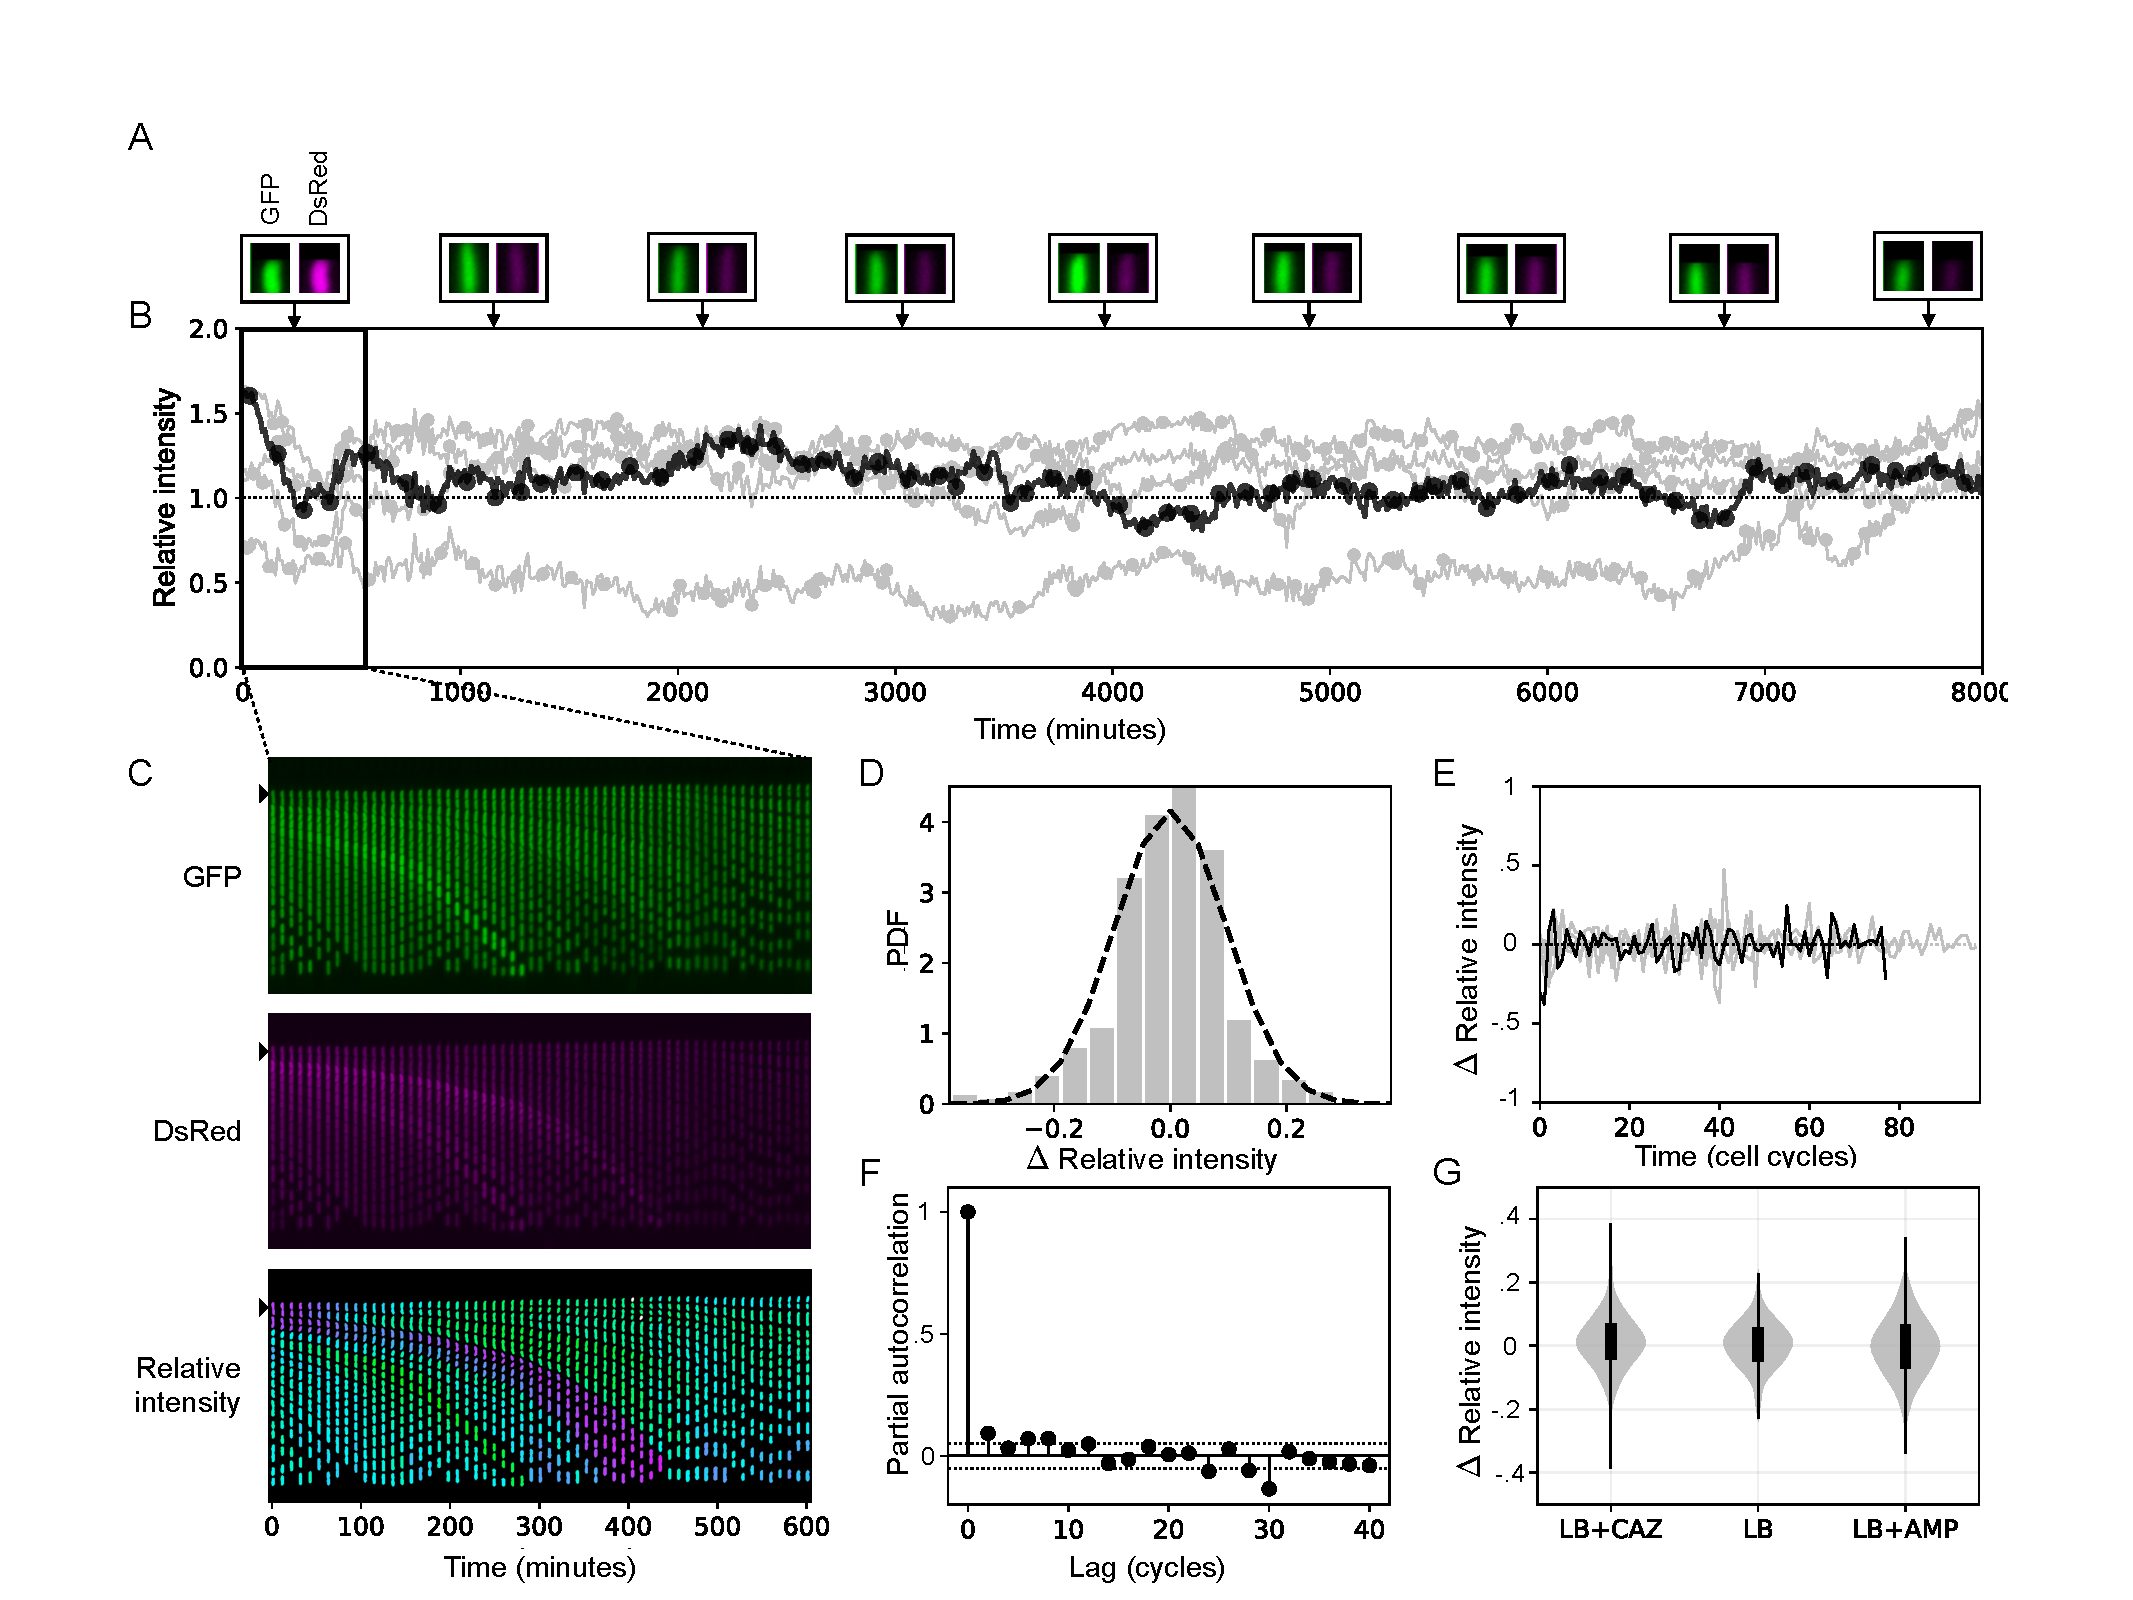
\includegraphics[width=.9\linewidth]{figures/Figure3.pdf}
\caption{ \small{ A) Mother cells at different time-points.  Note how the intensity in GFP and DsRed channels changes in time.  B) Time-series of relative intensity for individual cells in a long-term experiment. In black data obtained from the mother cell illustrated in A), while 4 other cells are shown in grey. Circles represent division events. C) Kymograph showing the progeny of the mother cell shown in A). From the images obtained in GFP (top) and DsRed (middle), we can use image processing to estimate the relative intensity of each cell (bottom).  D) Probability density function of the difference in relative fluorescence of an individual cell between consecutive frames.  This distribution can be approximated by a Normal distribution with mean near zero and $\sigma^2=0.096$.  E) $\Delta$ relative intensity as a function of time for cells shown in B).  F) Partial autocorrelation function of $\Delta$ relative intensity.  G) Distributions of $\Delta$ relative intensity are normally distributed.  A symmetric distribution suggests a random walk that is not correlated with the selective pressure imposed by the environment (left: ceftazidime, middle: drug-free, and right: ampicillin) }}
\label{fig:mother-machine}
\end{figure}
%%%%%%%%

%%%%%%%%%%%%%%%%%%%%%%%%%%%%%%%%%%%
\subsubsection{Intracellular plasmid dynamics is stochastic \blue{and not influenced by antibiotic selection}}

The benefit of mother-machine microfluidic devices is that they allow us to culture individual cells for hundreds of generations under the microscope, in contrast to microscope culture protocols which do not actively remove progeny during growth and therefore get rapidly saturated.  Multiple mother-machine devices have been proposed \cite{taheri2015single,long2013microfluidic}, but we will we use a dual-input mother machine\cite{Kaiser2018}, as it allows us to precisely control the concentration of antibiotic inside the microfluidic chip.  

First, we performed a long-term experiment consistent on introducing HT cells into the device and observing them for a period of 72 hours. 
We observed four device positions with $\sim 13$ microchannels per field of view, leading to $244\blue{,}249$ single-cell measurements, with mean fluorescent intensities of $212\pm 81 $ for GFP and $155\pm 51$ in DsRed, normalized \blue{relative intensity} of $1.42\pm 0.53$, and normalized \blue{absolute intensity} of $0.46\pm 0.14$. 
By acquiring images in multiple channels (GFP represented in green and DsRed in magenta) we can follow changes in fluorescence intensity between division events.  
\fig{Figure \ref{fig:mother-machine}A} shows a montage of mother cells at specific time-points, with their corresponding time-series represented in \fig{Figure \ref{fig:mother-machine}B} (black line corresponding to the cell illustrated in Figure \ref{fig:mother-machine}A, while grey lines show the relative intensity time-series obtained for other representative cells in the device). 
% 79,  73, 99,  83,  49 divisions  avg 76.6

It is important to highlight that time-series shown in \fig{Figure \ref{fig:mother-machine}B} are very long time-series ($72$ hours,  up to $99$ cell cycles), allowing us to quantify the difference in relative fluorescent exhibited by each cell at the moment of division and to estimate the difference in fluorescence between consecutive cell cycles, a quantity we refer to as {\em $\Delta$ relative intensity}.  \fig{Figure \ref{fig:mother-machine}E} shows how the time-series of $\Delta$ relative intensity produces increases in one fluorescent channel as frequently as increases in the other direction.
As a result, the difference between relative intensity values estimated in consecutive time-points is approximated by a Normal distribution with $\mu=0.00057$ a $\sigma^2=0.0092$ (see \fig{Figure \ref{fig:mother-machine}D}).

\fig{Figure \ref{fig:mother-machine}F} shows the partial autocorrelation function obtained for time-series of relative intensity in a drug-free environment. Note lags$>0$ are within the $95\%$ confidence interval, suggesting that changes in plasmid frequency are generated by an auto regressive process of first order, consistent with the tenet that random segregation and replication of plasmids are inherently stochastic processes.
Another interesting feature of our data is that intracellular plasmid diversity can be maintained for many generations in individual bacterial cells. Of course, phenotypic delay\cite{Sun2018} and fluorescent protein stability\cite{Balleza2018} could also stabilize fluorescence, but only for a few cell cycles. 

However, a consequence of the random segregation of plasmids is that there is a probability larger than zero of segregating plasmids unevenly between mother and daughter cells. In our experimental system, this would be reflected as large jumps in $\Delta$ relative intensity.  \fig{Figure \ref{fig:mother-machine}C} shows a kymograph obtained from a time-lapse movie (\fig{Supplementary Movie S1}), whereby the cell in the top of the channel (marked with a black triangle) corresponds to the time-series shown in \fig{Figure \ref{fig:mother-machine}B}.  Top and middle images correspond to GFP and DsRed channels, while the bottom image illustrates masks obtained after image segmentation, color-coded to represent the relative intensity value obtained after normalizing both fluorescent channels.  Note how, in general, fluorescence between mother and daughter cells appears to be correlated but, occasionally, a mother cell segregates plasmids unevenly upon division, producing daughter cells with different plasmid configurations (for example the magenta lineage in the kymograph). In the extreme scenario, HT inherits only plasmid of one type to the daughter cell, producing R12 or G1 cells with a probability that can be estimated from a binomial distribution. 

In summary, we have established that, as generally assumed by theoretical models of plasmid dynamics \cite{Ilhan2019,santer2019evolutionary,SanMillan2014,Rodriguez2018} segregation and replication of multicopy plasmids are noise-driven stochastic processes. Now we would like to evaluate if plasmid frequencies are under selection at the level of single cells.
To precisely control the concentration of antibiotics inside the microfluidic chip, we developed an automated pressure control system\cite{Ferry2011} that allows us to introduce different antibiotics into the device and quantify changes in intracellular plasmid frequency in response to environmental change.
So we introduced HT cells into the device and observed them for 15 hours previous to the introduction to the antibiotic following a ramp protocol: linearly increasing the concentration of antibiotic until reaching a lethal dose and maintaining that concentration constant until all cells are dead. 

When introducing ampicillin, we found that the distribution of $\Delta$ relative intensity remained symmetric with respect to zero, implying that AMP is not selecting for pBGT-1 plasmids at the level of individual cells.  We repeated this microfluidic experiment, now introducing CAZ to select for pBRT-12 plasmids, and confirmed that the shape of the resulting distribution of $\Delta$ relative intensity was not skewed towards DsRed.  \fig{Figure \ref{fig:mother-machine}G} illustrates violin plots of $\Delta$ relative intensity for different selective pressures. Note that, independently of the environmental condition, the shape of the distributions is qualitatively the same (for AMP a Normal distribution with $\mu=-0.00073$, $\sigma^2=0.0129$, and for CAZ with $\mu=0.01298$, $\sigma^2=0.0098$). We performed a non-parametric Kolmogorov-Smirnov normality test comparing each distribution against a theoretical Normal distribution with the corresponding $\mu$ and $\sigma^2$ ($H_0:$ the distribution is not Normal,  p-values$=(0.527,\ 0.493,\ 0.8017)$ for LB, AMP, and CAZ respectively). In conclusion, regardless the selection regime, the distribution of $\Delta$ relative intensities follows a Normal distribution, indicating that changes in relative abundances of different plasmids in single-cells are driven by random noise and not by selection.

%%%%%%%%%%%%%%%%%%%%%%%%%%%%%%%%%%%

\subsection{Using microchemostats to study plasmid dynamics in bacterial colonies}

We have established that selection can modulate plasmid frequency distributions of heterozygous bacterial populations, and also that intracellular plasmid dynamics is a noise-driven process that does not seem to be affected by selection.   Therefore we argue that the shift in fluorescence observed at a population-level must be a consequence of antibiotics selecting for subpopulations with different plasmid configurations. To evaluate this hypothesis and to study the effect on selection in heterozygous populations, we used a different microfluidic device that provides high-throughput time-resolved information about thousands of individual cells simultaneously.

Microchemostats are designed to cultivate bacterial colonies for long periods of time in controlled and well-mixed environments \cite{moffitt2012single,mondragon2011entrainment,lopatkin2016antibiotics,li2019dissecting}. In particular, here we use a microchemostat adapted from \cite{mondragon2011entrainment} that consists of two parts: the signal generator and the cell confinement region. In the confinement section there are $48$ rectangular chambers distributed in four rows. Each containment chamber measures $40 \times 50 \times 0.95 \mu m^3$, with two sides open to a large channel where media is introduced and cells are washed out of the device. Since {\em E. coli} cells are approximately $1 \mu m$ in diameter, confining them in these microfluidic traps allows the simultaneous observation of a colony of approximately $500$ cells in the same focal plane. Furthermore, as with the dual-input mother machine, we can use a signal generator to dynamically control the extracellular concentration of antibiotics.


%%%%%%%%
%%Figure 4 -Michochemostat
\begin{figure}[ht!]
\centering
\includegraphics[width=.8\linewidth]{figures/Figure4.pdf}
\caption{ \small{ A) Plasmid fraction as a function of time for a population of HT cells exposed to a ramp of CAZ.  B) Polar distribution of cells at the end of the experiment. The black arrow represents changes in the mean plasmid frequency of the population, before and after antibiotic exposure. C) Montage of microscopy images (GFP channel in green, and DsRed in magenta, with both channels overlaid).  D) Fraction of cells with a higher proportion of pBGT-1 plasmids is increased when AMP is introduced into the device. E-F) Population-level distribution at the end of the experiment.  Note how the black arrow points towards higher values of GFP, suggesting that the mean plasmid frequency of the population moved towards cells carrying relatively more copies of pBGT-1.}}
\label{fig:microchemostat}
\end{figure}
%%%%%%%%

%%%%%%%%%%%%%%%%%%%%%%%%%%%%%%%%%%%
\subsubsection{Heteroplasmy is unstable in environments with constant selection} 

\fig{Figure \ref{fig:microchemostat}} illustrates an experiment where a population of HT cells was cultured in drug-free media for 6 hours, followed by the introduction of antibiotics using a linear ramp. When drug concentration reached a lethal dose ($4\ mg/ml$ for AMP and $8\ \mu g/ml$ for CAZ), the concentration of antibiotics was maintained constant until all cells were dead (see \fig{Supplementary Movies S2 and S3}).
\fig{Figure \ref{fig:microchemostat}C} shows montages of selected traps at different time-points (CAZ in the top and AMP at the bottom).  

We used our image processing pipeline to analyze all traps containing cells growing exponentially after growing overnight inside the device.  As in the flow cytometry data, we measured the relative and absolute intensity of each individual cell but, as opposed to flow cytometry data, our microchemostat allows us to track cells in time and perform lineage reconstruction.  In particular, we obtained $557$ lineages, corresponding to $5\blue{,}870$ cells in the CAZ experiment and 498 lineages of $5\blue{,}754$ cells for AMP.  
Of course, as the colony is growing exponentially, most cells are pushed out of the trap and washed out of the device, so only a few lineages were observed from start to end of the experiment. We recovered $48$ complete lineages for CAZ and $46$ for AMP and, consistent with the results shown in \fig{Figure \ref{fig:mother-machine}G}, the resulting time-series were not correlated with the selective pressure imposed by the environment.

Now, by clustering the population according to their relative fluorescent intensity, we determined the fraction of cells with different plasmid frequencies.
As illustrated in \fig{Figure \ref{fig:microchemostat}A}, exposing a population of HT cells to CAZ produces an increase in the fraction of cells with high levels of DsRed and low intensity values of GFP, implying that selection favours cells with a higher proportion of pBRT-12 plasmids.
The black arrow in the polar distributions shown in \fig{Figure \ref{fig:microchemostat}B} denotes changes in the mean relative intensity of the population after 6 hours of exposure to CAZ and, as expected, points towards R12. 
In contrast, when introducing AMP into the device, the fluorescent intensity distribution appeared to be shifted towards GFP, consequence of G1 cells being positively selected for, a feature that can be seen in \fig{Figure \ref{fig:microchemostat}D} and in the polar distribution shown in \fig{Figure \ref{fig:microchemostat}E}.

Notably, the shift is larger when using CAZ than in the presence of AMP. This is explained by $bla_{\text{TEM-1}}$ providing partial resistance to AMP and therefore the relative fitness (and thus the rate of fixation) is larger for R12 in ceftazidime than G1 in ampicillin.
In any case, HT cells reduced in frequency and are destined to be outcompeted by homozygous subpopulations: R12 if using CAZ or G1 in an AMP environment.  This is consistent with previous studies showing that heteroplasmy is unstable in constant environmental conditions \cite{Rodriguez2018}. It has also been reported that fluctuating environments can stably maintain intracellular genetic diversity for long-time intervals, so in the following section we will evaluate this hypothesis using microchemostats.

%%%%%%%%%%%%%%%%%%%%%%%%%%%%%%%%%%%
\subsubsection{Fluctuating environments stabilize genetic diversity}

By alternating both antibiotics periodically, we experimentally explored if fluctuating environmental conditions can stabilize plasmid-mediated heterozygosis.
Specifically, we introduced HT cells into the device and observed them in LB for about 3 hours before introducing antibiotics.
To implement a fluctuating selection regime, we generated a sinusoidal signal of period 2 hours such that, when CAZ concentration is at 100\%, then AMP is at 0\%, and vice versa, as illustrated in \fig{Figure 5C} (in green the concentration of AMP and in magenta of CAZ, both normalized to the same critical concentrations used before). 
We diluted a fluorescent dye to one of the antibiotic inputs to calibrate the height of the syringes, but this also allowed us to use the fluorescent microscope to validate that cells are exposed to the expected proportion between both antibiotics. Magenta dots represent DsRed measurements in a \blue{cell}-free area of the device and correspond very precisely with the drug-deployment protocol sent by the signal generator.


%%%%%%%%
%%Figure 5 -Fluctuating environments
\begin{figure}[ht!]
\centering
    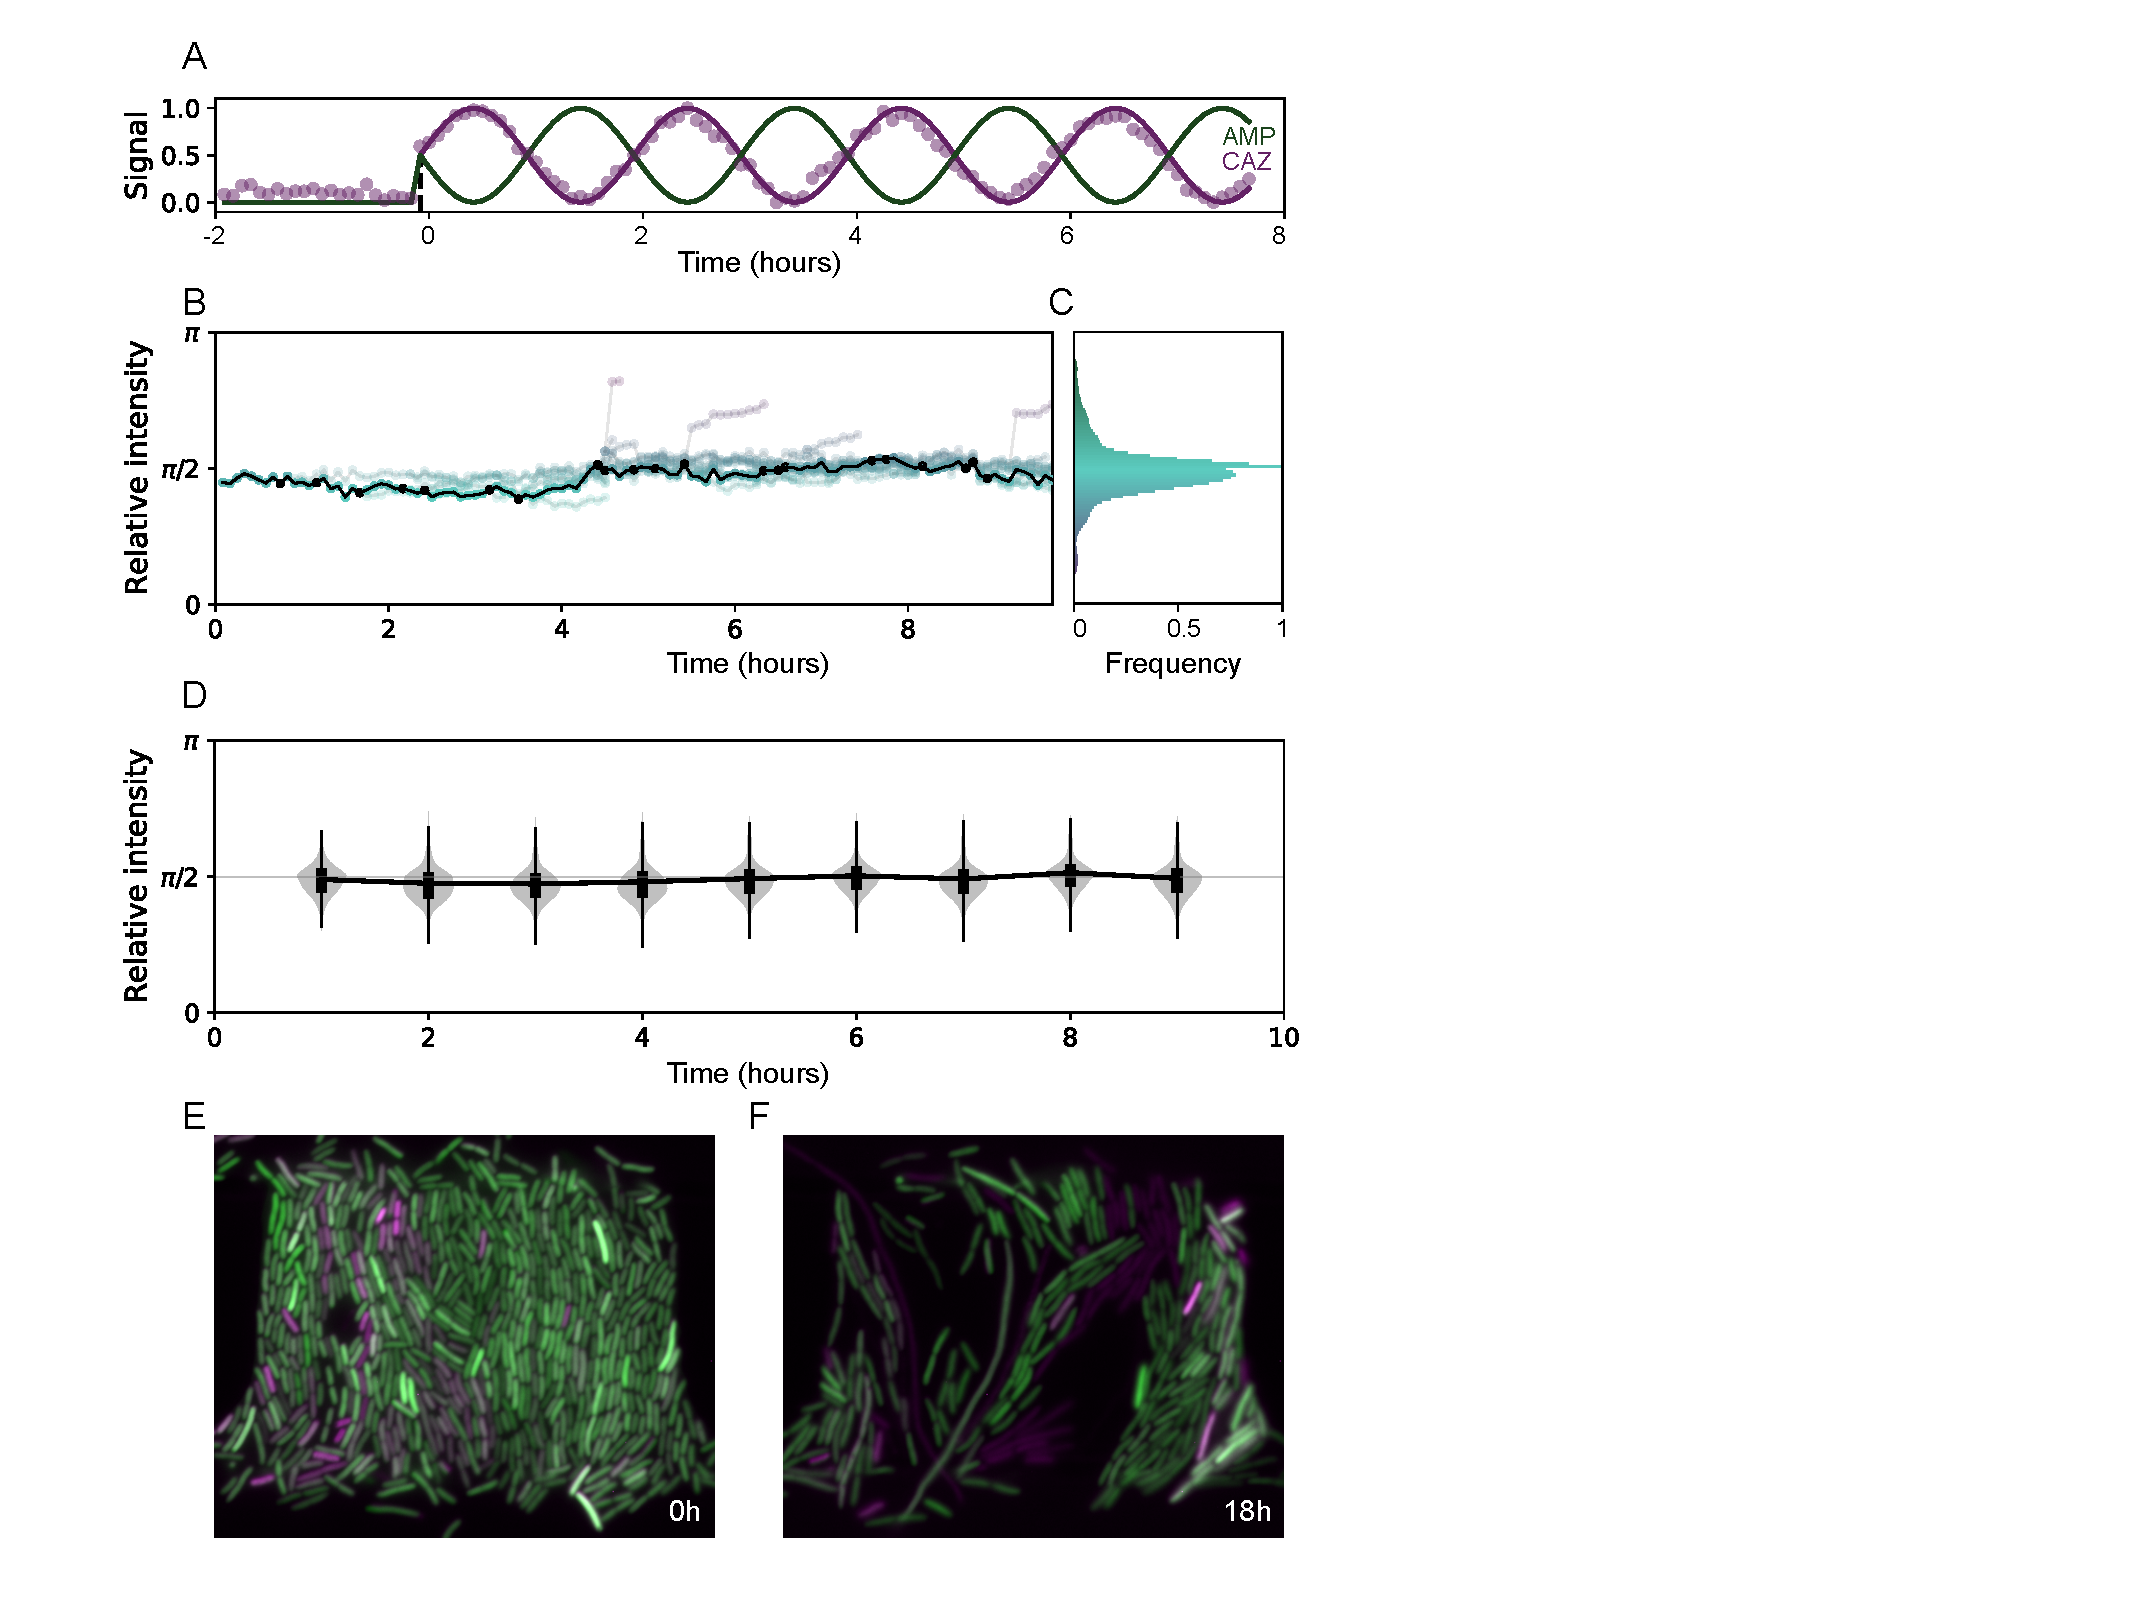
\includegraphics[width=0.7\linewidth]{figures/Figure5.pdf}
\caption{ \small{A) Oscillatory drug deployment protocol consisting on CAZ (magenta) and AMP (green) being alternated every two hours. Magenta circles correspond to measured values of fluorescent dye also introduced into the device together with CAZ.  B) Black line represents a single-cell lineage obtained from a time-lapse movie of a microchemostat.  Black circles represent division events and relative fluorescence of daughter cells is illustrated in cyan.  C) Relative fluorescent distribution obtained after 18 hours of exposure to fluctuating CAZ and AMP selective pressures.  D) Population-level relative intensity distributions at different time-points.  A consequence of alternating selection for both alleles is that intermediate values of relative fluorescence are maintained for long time periods, suggesting that genetic diversity can be stabilized in fluctuating environmental conditions. E) Microscopy images at the beginning (left) and at the end (right) of the experiment. Note how, after 18 hours of fluctuating selection, the resulting population is composed of R12 and G1 cells, but also of HT cells.}}
\label{fig:sine}
\end{figure}

\fig{Figure 5B} shows a lineage reconstruction where the black line corresponds to an individual cell observed for the complete duration of the experiment, while other cells in the lineage are illustrated in cyan.  Note how, as previously shown in the mother-machine, the intracellular plasmid dynamics appears to be random and is not correlated with the environmental signal.  A consequence of the random segregation and replication of plasmids is that, after only a few generations, the distribution of alleles in the population presents a large variance, as shown in \fig{Figure 5C}.

As we have previously argued, we cannot make inferences about the stability of plasmid-mediated heterozygosis from single-cell data. So we included the remaining cells to our analysis and estimated relative intensity distributions at different time-points.  \fig{Figure 5D} shows violin plots representing the distribution estimated every hour.  As opposed to the constant drug environment discussed previously, in the alternating selection regime, the mean relative intensity is centered around HT throughout the duration of the experiment (although the variance increases in time).  \fig{Figures 5E} and \fig{5F} show composite images at $t=0$ and at $t=18$ hours, extracted from Supplementary Movie S4, revealing the presence of G1 and R12 cells at the end of the experiment and, crucially, of cells still bearing both plasmids. 

%\doing{We repeated this experiment for different periods and also found that PMH was stable}



%%%%%%%%%%%%%%%%%%%%%%%%%%%%%%%%%%%
%%%%%%%%%%%%%%%%%%%%%%%%%%%%%%%%%%%
\section{\blue{Discussion}}

\blue{The rate at which pathogenic bacteria evolve resistance to antibiotics is dramatically decreasing the efficacy of current antimicrobial treatments. It may seem a surprising statement but, after more than a century of using antimicrobials in the clinic, some of the evolutionary forces that drive the emergence and spread of drug resistance in pathogenic bacteria are still poorly understood. For instance, most of our understanding of drug resistance adaptation assumes that clonal populations growing in constant environments present similar susceptibility and resistance profiles to antibiotics, while actually clinical isolates can present a high degree of heterorresistance generated, in many cases, by heterogeneous expression of plasmid-borne resistance genes.\cite{andersson2019mechanisms}. }

\blue{In a previous paper \cite{Rodriguez2018}, we used mathematical modelling and experimental evolution to argue that multi-copy plasmids can provide a platform to increase intracellular genetic diversity and, in consequence, enhance the probability of survival to dynamic environmental conditions.}
\blue{Here we used microfluidics and fluorescence microscopy to study, with single-cell resolution, the effect of selection in the relative abundance of incompatible plasmids carrying different versions of an antibiotic resistance gene and a fluorescent marker.} 
\blue{As expected, in the absence of selection, the stochastic nature of plasmid replication and segregation renders plasmids unstable and decreases allele frequency in the population.  In contrast, positive selection for plasmid-encoded genes stabilizes plasmids at high copy-numbers, increasing the frequency of the corresponding allele and promoting resistance to the antibiotics used. }

\blue{Of course, natural environments are not constant but alternate selection between subpopulations with different genetic configurations. Therefore, in dynamic environments, it may be optimal for bacterial populations to present genetic heterogeneity, thus increasing the probability that some individuals are pre-adapted to future environmental conditions\cite{Ackermann2015}. 
Indeed, }in agreement with previous laboratory studies\cite{Rodriguez2018}, we showed that fluctuating selection  - in this case, alternating the extracellular concentration of different $\beta$-lactam antibiotics - \blue{maintained intracellular genetic diversity in the population for longer than constant environmental regimes. }

\blue{Although previous studies have successfully deployed a combination of experimental evolution \cite{maclean2015,harrison2012,holloway2007}, genome sequencing \cite{Harrison2015,SanMillan2014,porse2016survival} and mathematical modeling \cite{SanMillan2014,Wein2019,santer2019evolutionary,yurtsev2013bacterial,stewart1977population} to evaluate the population dynamics that emerge in response to different environmental conditions,} the intrinsic resolution of flow cytometers and qPCR machines do not allow us to dissect \blue{stochastic} plasmid dynamics (generated by randomly replicating and partitioning plasmids) from \blue{deterministic} population-level effects (e.g. differences in relative fitness associated with expressing multiple alleles).  So, in this paper, we used single-cell microfluidics to generate high-throughput fluorescent intensity data of heterozygous bacterial populations exposed to a range of selective regimes.

\blue{In particular, we used computer vision algorithms to analyze} time-lapse movies acquired in multiple fluorescence channels, allowing us to characterize the allele distribution in the population in terms of the relative and absolute fluorescent intensities of its constituent cells. This allowed us to evaluate directly the contribution of selection and random genetic drift in the rate of fixation and extinction of different plasmid variants.  We showed, using a mother-machine to restrain individual cells and follow them for very long periods, that changes in plasmid frequency are the consequence of a noise-driven process that is not correlated with the direction and strength of selection imposed by the environment.  

We conclude by arguing that imaging and microfluidics can provide a potentially useful approach to study \blue{the interaction between intracellular plasmid dynamics and selection imposed by the environment,} and therefore could be used to increase our understanding of the complex interaction between mobile genetic elements, their bacterial hosts, and the environment.

%%%%%%%%%%%%%%%%%%%%%%%%%%%%%%%%%%%%%%%%%%% 
\section*{Supplementary material}

\textbf{Supplementary Movie S1.} Time-lapse movie of individual HT cells growing in LB media inside a mother-machine microfluidic device.

\textbf{Supplementary Movie S2.} Time-lapse movie of a colony composed of HT cells exposed to a ramp of AMP inside a microchemostat.

\textbf{Supplementary Movie S3.} Time-lapse movie of a colony composed of HT cells exposed to a ramp of CAZ inside a microchemostat.

\textbf{Supplementary Movie S4.} Time-lapse movie of a colony composed of HT cells exposed to an oscillatory regime that cycles between AMP and CAZ every two hours.
%%%%%%%%%%%%%%%%%%%%%%%%%%%%%%%%%%%%%%%%%%%
%%%%%%%%%%%%%%%%%%%%%%%%%%%%%%%%%%%%%%%%%%% 
\section*{Acknowledgements}

We are grateful to Craig MacLean, Octavio Mondrag\'on-Palomino, David Zamorano and members of the Fuentes-Hern\'andez and Pe\~na-Miller groups for helpful discussions, comments, and suggestions. Also to Jose Escudero for generous gifts of strains and plasmids.
We are also thankful with Andr\'es Saralegui Amaro from Laboratorio Nacional de Microscop\'ia Avanzada for assistance using the flow cytometer. JCRH is a doctoral student in Programa de Doctorado en Ciencias Biom\'edicas, Universidad Nacional Aut\'onoma de M\'exico, and received fellowship 59691 from CONACYT. 
This work was supported by a Newton Advanced Fellowship awarded by the Royal Society (NA140196) and by CONACYT (Ciencia B\'asica grant A1-S-32164), both awarded to RPM. AFH and RPM were also supported by PAPIIT-UNAM (grants IA201418 and IN209419, respectively). ASM is supported by a Miguel Servet Fellowship (MS15-00012). JRB is a recipient of a Juan de la Cierva-Incorporaci\'on Fellowship (IJC2018-035146-I). 

%%%%%%%%%%%%%%%%%%%%%%%%%%%
\small
\bibliography{refs}

\end{document}